\section{Ultrasound Fetal Brain Images Synthesis}

%%%%%%%%%%%%%%%%%%%%%%%%%%%%%%%%%%%%%%%%%%%%
\subsection{Clinical background and research aims}
\begin{frame}
  \frametitle{Table of Contents}
  \tableofcontents[currentsubsection]
\end{frame}


%%%%%%%%%%%%%%%%%%%%%%%%%%%%%%%%%%%%%%%%%%%%%%%%%%%%%%%%
{
\paper{
Wright-Gilbertson M. 2014 in PhD thesis; \url{https://en.wikipedia.org/wiki/Gestational_age}; 
National-Health-Service 2021. Screening for down’s syndrome, edwards’ syndrome and patau’s syndrome. \url{https://www.nhs.uk/pregnancy/your-pregnancy-care} 
}

\begin{frame}{Dating US scan (12-week scan)}{Clinical background}
      \begin{figure}
        \centering
        \includegraphics[width=1.0\textwidth]{us-12-week-scan-dating-scan/outputs/drawing-v02}
        % \caption{The sonographer-probe-patient control system}
      \end{figure}
\end{frame}
}


%%%%%%%%%%%%%%%%%%%%%%%%%%%%%%%%%%%%%%%%%%%%%%%%%%%%%%%%
{
\paper{
International Society of Ultrasound in Obstetrics and  Gynecology Education Committee. 
"Sonographic examination of the fetal central nervous system: guidelines for performing the'basic examination'and the'fetal neurosonogram'." 
Ultrasound in obstetrics and gynecology: the official journal of the International Society of Ultrasound in Obstetrics and Gynecology 29, 
no. 1 (2007): 109-116.
}

\begin{frame}{Fetal US brain scans}{Clinical background}
      \begin{figure}
        \centering
        \includegraphics[width=1.0\textwidth]{us-14-16-week-scan/outputs/drawing-v00}
        % \caption{The sonographer-probe-patient control system}
      \end{figure}
\end{frame}
}





%%%%%%%%%%%%%%%%%%%%%%%%%%%%%%%%%%%%%%%%%%%%%%%%%%%%%%%%
{
\paper{
Sciortino et al. in Computers in Biology and Medicine 2017 https://doi.org/10.1016/j.compbiomed.2017.01.008; 
He et al. in Front. Med. 2021 https://doi.org/10.3389/fmed.2021.729978
Thomas L. A. van den Heuvel et al. https://hc18.grand-challenge.org/
Burgos-Artizzu, X et al. (2020). FETAL PLANES DB: Common maternal-fetal ultrasound images [Data set]. In Nature Scientific Reports (1.0, Vol. 10, p. 10200). Zenodo. https://doi.org/10.5281/zenodo.3904280
}
\begin{frame}{Challenges in Ultrasound biometric measurements}{Clinical background}

\begin{itemize}
% \item Operator dependant
% \item Position of the fetus
% \item Similar morphological and echogenic characteristics in the US image
% \item Threshold selection of the binary masks 
% \item Few public datasets are available [Thomas et. al 2018; Burgos-Artizzu et al. 2010]
%https://www.nature.com/articles/jhg200888
\item intra-view variability of imaging equipment and inter-observer variability of sonographer skills,
\item availability of expert clinicians or trained technicians to collect, to select, to classify and to validate regions of interest,
\item the cost of acquisition of clinical data as it requires expensive imaging equipment and experts for data collection and validation
\item the insufficient and limited amount of clinical data,
\item data accessibility due to patient privacy or protection of personal health information,
\end{itemize}

\end{frame}
}



%\section{Research aims}
%\begin{frame}
%  \frametitle{Table of Contents}
%  \tableofcontents[currentsection]
%\end{frame}



%%%%%%%%%%%%%%%%%%%%%%%%%%%%%%%%%%%%%%%%%%%%%%%%%%%%%%%%
{
%\paper{Wright-Gilbertson M. 2014 in PhD thesis}
\begin{frame}{Research aims}

\bigSizeFont
\begin{itemize}
\item Investigate and implement GAN-based and Diffusion-based models to synthetise realistic high-quality fetal ultrasound images
% of three fetal planes: trans-thalamic; trans-ventricular and trans-cerebellum.
% \item Propose and apply methods to evaluate quantitative and qualitative images of abnormal cases [High-risk]
\end{itemize}

\end{frame}
}


\subsection{Datasets of Fetal Brain Ultrasound Images}
\begin{frame}
  \frametitle{Table of Contents}
  \tableofcontents[currentsubsection]
\end{frame}


%%%%%%%%%%%%%%%%%%%%%%%%%%%%%%%%%%%%%%%%%%%%%%%%%%%%%%%%
{
\paper{
Burgos-Artizzu, X et al. (2020). FETAL PLANES DB: Common maternal-fetal ultrasound images [Data set]. In Nature Scientific Reports (1.0, Vol. 10, p. 10200). Zenodo. https://doi.org/10.5281/zenodo.3904280
}

\begin{frame}{TransThalamic}{Datasets of Fetal Brain Ultrasound Images}
      \begin{figure}
        \centering
        \includegraphics[width=1.0\textwidth]{fetal-planes-dataset-TransThalamic/outputs/drawing-v00}
        %\caption{}
      \end{figure}
\end{frame}
}

%%%%%%%%%%%%%%%%%%%%%%%%%%%%%%%%%%%%%%%%%%%%%%%%%%%%%%%%
{
\paper{
Burgos-Artizzu, X et al. (2020). FETAL PLANES DB: Common maternal-fetal ultrasound images [Data set]. In Nature Scientific Reports (1.0, Vol. 10, p. 10200). Zenodo. https://doi.org/10.5281/zenodo.3904280
}

\begin{frame}{TransCerebellum Plain}{Datasets of Fetal Brain Ultrasound Images}
      \begin{figure}
        \centering
        \includegraphics[width=1.0\textwidth]{fetal-planes-dataset-TransCerebellum/outputs/drawing-v00}
        %\caption{}
      \end{figure}
\end{frame}
}





%%%%%%%%%%%%%%%%%%%%%%%%%%%%%%%%%%%%%%%%%%%%%%%%%%%%%%%%
{
\paper{
Burgos-Artizzu, X et al. (2020). FETAL PLANES DB: Common maternal-fetal ultrasound images [Data set]. In Nature Scientific Reports (1.0, Vol. 10, p. 10200). Zenodo. https://doi.org/10.5281/zenodo.3904280
}

\begin{frame}{TransVentricular Plane}{Datasets of Fetal Brain Ultrasound Images}
      \begin{figure}
        \centering
        \includegraphics[width=1.0\textwidth]{fetal-planes-dataset-TransVentricular/outputs/drawing-v00}
        %\caption{}
      \end{figure}
\end{frame}
}






\subsection{Machine Learning Pipeline}
\begin{frame}
  \frametitle{Table of Contents}
  \tableofcontents[currentsubsection]
\end{frame}

%%%%%%%%%%%%%%%%%%%%%%%%%%%%%%%%%%%%%%%%%%%%%%%%%%%%%%%%
{
% \paper{Private github repository: \url{https://github.com/xfetus/synthetic-foetuses​ }}
\begin{frame}{Machine Learning Pipeline}{Fetal US imaging synthesis with GANs}
      \begin{figure}
        \centering
        \includegraphics[width=1.0\textwidth]{machine-learning-pipeline/outputs/drawing-v01}
        %\caption{}
      \end{figure}
\end{frame}
}



\subsection{Methods}
\begin{frame}
  \frametitle{Table of Contents}
  \tableofcontents[currentsubsection]
\end{frame}


%%%%%%%%%%%%%%%%%%%%%%%%%%%%%%%%%%%%%%%%%%%%%%%%%%%%%%%%
{
\paper{
M. Iskandar et al.  "Towards Realistic Ultrasound Fetal Brain Imaging Synthesis" in MIDL2023
\faGithub \, \url{https://github.com/budai4medtech/midl2023}
}
\begin{frame}{Image Quality Assessment}{Methods}
      \begin{figure}
        \centering
        \includegraphics[width=1.0\textwidth]{Image-Quality-Assessment/outputs/drawing-v00}
%         \caption{(a) DCGAN arquitecture, loss functions for DC-GANs and batches of synthetic fetal head images,
% 		(b) FASTGAN arquitecture and batches of synthethic fetal head images}
      \end{figure}
\end{frame}
}



%%%%%%%%%%%%%%%%%%%%%%%%%%%%%%%%%%%%%%%%%%%%%%%%%%%%%%%%
{
\paper{
M. Iskandar et al.  "Towards Realistic Ultrasound Fetal Brain Imaging Synthesis" in MIDL2023
\faGithub \, \url{https://github.com/budai4medtech/midl2023}
}
\begin{frame}{Diffusion-Super-Resolution-GAN (DSR-GAN)}{Methods}
      \begin{figure}
        \centering
        \includegraphics[width=1.0\textwidth]{Diffusion-Super-Resolution-GAN/outputs/drawing-v00}
%         \caption{(a) DCGAN arquitecture, loss functions for DC-GANs and batches of synthetic fetal head images,
% 		(b) FASTGAN arquitecture and batches of synthethic fetal head images}
      \end{figure}
\end{frame}
}



%%%%%%%%%%%%%%%%%%%%%%%%%%%%%%%%%%%%%%%%%%%%%%%%%%%%%%%%
{
\paper{
M. Iskandar et al.  "Towards Realistic Ultrasound Fetal Brain Imaging Synthesis" in MIDL2023
\faGithub \, \url{https://github.com/budai4medtech/midl2023}
}
\begin{frame}{Transformer-based-GAN}{Methods}
      \begin{figure}
        \centering
        \includegraphics[width=1.0\textwidth]{Transformer-based-GAN/outputs/drawing-v00}
%         \caption{(a) DCGAN arquitecture, loss functions for DC-GANs and batches of synthetic fetal head images,
% 		(b) FASTGAN arquitecture and batches of synthethic fetal head images}
      \end{figure}
\end{frame}
}



\subsection{Results}
\begin{frame}
  \frametitle{Table of Contents}
  \tableofcontents[currentsubsection]
\end{frame}


%%%%%%%%%%%%%%%%%%%%%%%%%%%%%%%%%%%%%%%%%%%%%%%%%%%%%%%%
{
\paper{
M. Iskandar et al.  "Towards Realistic Ultrasound Fetal Brain Imaging Synthesis" in MIDL2023
\faGithub \, \url{https://github.com/budai4medtech/midl2023}
}
\begin{frame}{Experiments: Design and results (256x256 pixel images)}
      \begin{figure}
        \centering
        \includegraphics[width=0.9\textwidth]{results-only-images/outputs/drawing-v00}
      \end{figure}
\end{frame}
}


%%%%%%%%%%%%%%%%%%%%%%%%%%%%%%%%%%%%%%%%%%%%%%%%%%%%%%%%
{
\paper{
M. Iskandar et al.  "Towards Realistic Ultrasound Fetal Brain Imaging Synthesis" in MIDL2023
\faGithub \, \url{https://github.com/budai4medtech/midl2023}
}
\begin{frame}{Experiments: Design and results}
      \begin{figure}
        \centering
        \includegraphics[width=1.0\textwidth]{results/outputs/drawing-v00}
        \caption{
        Results from Diffusion-Super-resolution-GAN (DSR-GAN) and transformerbased-GAN (TB-GAN):
        (a) Training losses for Generator and Discriminator networks,
        (b) FID scores, and
        (c) 256x256 pixel size trans-cerebellum images of two randomised batches (B1, B2) of real and synthesised (DSR-GAN and TB-GAN)
		}
      \end{figure}
\end{frame}
}



%%%%%%%%%%%%%%%%%%%%%%%%%%%%%%%%%%%%%%%%%%%%%%%%%%%%%%%%
{

\paper{
(a) Ho et al. 2020 "Denoising Diffusion Probabilistic Models" https://arxiv.org/abs/2006.11239
(b) Fiorentino et al. 2022 "A Review on Deep-Learning Algorithms for Fetal Ultrasound-Image Analysis" https://arxiv.org/abs/2201.12260
(c) Burgos-Artizzu, X et al. (2020). FETAL PLANES DB: Common maternal-fetal ultrasound images [Data set]. In Nature Scientific Reports (1.0, Vol. 10, p. 10200). Zenodo. https://doi.org/10.5281/zenodo.3904280
}

\begin{frame}{Fetal imaging synthesis with difussion models}{Future work}
      \begin{figure}
        \centering
        \includegraphics[width=1.0\textwidth]{future-work/outputs/drawing-v00}
        %\caption{ }
      \end{figure}
\end{frame}


}


%%%%%%%%%%%%%%%%%%%%%%%%%%%%%%%%%%%%%%%%%%%%%%%%%%%%%%%%
{

\paper{
M. Iskandar et al.  "Towards Realistic Ultrasound Fetal Brain Imaging Synthesis" in MIDL2023
\faGithub \, \url{https://github.com/budai4medtech/midl2023}
}

\begin{frame}{\faGithub \, GitHub repository: github.com/budai4medtech/midl2023}
      \begin{figure}
        \centering
        \includegraphics[width=1.0\textwidth]{github-repository/outputs/drawing-v00}
        %\caption{ }
      \end{figure}
\end{frame}


}



